\documentclass[12pt, twoside]{report}
\usepackage[a4paper,left=2cm, right=2cm, top=3cm,bottom=2cm]{geometry}
\usepackage[utf8]{inputenc}

\usepackage[english]{babel}
\usepackage{amsmath}
\usepackage{graphicx}
\usepackage{textcomp}
\usepackage{parskip}
\usepackage[colorinlistoftodos]{todonotes}
\usepackage{csquotes}
\usepackage{float}
\usepackage[backend=biber,style=ieee]{biblatex}
\usepackage{hyperref}
\usepackage{graphicx}
\usepackage{epsfig}
\usepackage{caption}
\usepackage{ragged2e}
\usepackage{subcaption}
\usepackage[singlespacing]{setspace}
\usepackage{hyperref}
\usepackage[utf8]{inputenc}
\usepackage[backend=biber,style=ieee]{biblatex}

\usepackage{biblatex}

%\addbibresource{friedt.bib}
\addbibresource{OCT_ref.bib}
\setlength {\marginparwidth }{2cm} 

%Chapter and name in the same line
\usepackage{titlesec}
\titleformat{\chapter}[hang] 
{\normalfont\huge\bfseries}{\chaptertitlename\ \thechapter:}{1em}{} 

\titleformat{\chapter}[display]
  {\normalfont\bfseries}{}{0pt}{\Huge}
  


\begin{document}

\begin{titlepage}

\newcommand{\HRule}{\rule{\linewidth}{0.5mm}}
\center 

\textsc{\LARGE Université Bourgogne Franche-Comté}\\[1.5cm] 
\textsc{\Large Master 1 in Smart Integrated Systems}\\[0.5cm] 

\HRule \\[0.4cm]
{ \huge \bfseries Porting GNU Radio to Buildroot: application to an embedded digital
network analyzer}\\[0.4cm] 
\HRule \\[1.5cm]


\includegraphics[scale=0.3]{logo_ubfc.png}\\[1cm]

\begin{center}
\begin{tabular}{ c   |   c } 
   
    Grover ARUQUIPA & \normalsize \href{mailto:grover.grover_aruquipa_aruquipa@edu.univ-fcomte.fr}{grover.grover \textunderscore aruquipa \textunderscore aruquipa@edu.univ-fcomte.fr}
    %Opcion 2:
    %ARUQUIPA Grover & \normalsize \href{mailto:grover.grover_aruquipa_aruquipa@edu.univ-fcomte.fr}{grover.grover \textunderscore aruquipa \textunderscore aruquipa@edu.univ-fcomte.fr}\\
    %RIVERA Carlos &  \normalsize \href{mailto:carlos_manuel.rivera_aguilar@edu.univ-fcomte.fr}{carlos\textunderscore manuel.rivera\textunderscore aguilar@edu.univ-fcomte.fr}
\end{tabular}
\end{center}

\vfill
{\large \today}\\[1cm] 
\vfill 

\end{titlepage}
 

%\thispagestyle{empty}
%\tableofcontents
%\listoffigures
\pagebreak



\pagebreak

\chapter{Abstract}
This work presents the development of a network analyzer application based on GNU Radio, a brief exploration of the state of the art regarding this field of development is presented, previous concepts that support the implementation of the system are developed, additionally a technical part is shown in the which specifies the sections of great importance for obtaining the results presented in this work. Finally, a section of conclusions is presented where a brief analysis and study of future perspectives attached to this work is presented.the codes and references are correctly attached in the footnotes and bibliography correctly for analysis and replication if necessary.\\
\newline

\textbf{Github Reposity:} \textit{\url{https://github.com/GroverAruquipa/Embedded_digital_network_analyzer.git}}


\setcounter{page}{1}
\chapter{Introduction}



\section{State of the Art}
Radio frequency technology is widely used in different applications,  everyday and in the engineering fields, in \cite{Valerio2008}-\cite{Valerio2008a} the importance of the diffusion of SDR \textit{Software Defined Radio} in different systems is pointed out as Soc's \textit{System on Chip} based on FPGA, the author shows an approximation to the current state of development of radio frequency applications through SDR, it is clearly explained how GNURadio is expected to become an open source standard in radio frequency research paradigms.\\
On the other hand, regarding the new application trends of GNU-Radio, in \cite{Lavric2021}  the author presents a work on the implementation of GNURadio with LoraWan for high volumes of data, managing to scale the GNU Radio paradigm to other fields. Similarly in \cite{White2017} the author uses GNU-Radio in the control of a telescope in order to improve his results, highlighting the advantages of GNU-Radio for this type of applications such as the friendly use of the interface and the growing community.\\
Additionally, another interesting work presented in \cite{OShea2016} the author shows the use of deep neural networks in the evaluation of different sets of public data and an implementation of GNU-Radio taking advantage of the potential of both fields for tasks such as modulation recognition, signal compression and the implementation of Reinforcement learning for signal manipulation, thus showing the synergy between both fields.\\
Finally, the authors in \cite{Marshall2021}-\cite{Mladenov2022} a communication implementation of a ground system with a cube-sat is shown, evaluating the robustness of the implementation and showing a successful testing of the program, in the same way the author points out a great flexibility for the use of GNU-Radio and also highlights the robustness due to the successful recovery of cubesat data.\\
On the other hand, regarding direct or similar approaches, the closest field for measuring the success of this work is the educational area, in this way \cite{Zabootny2020} presents its platform of frequency teaching based on GNU-Radio and HackRFOne, the author presents direct metrics based on teaching impact that do not align with this work, moreover as reference Jean-Michel Friedt in his work \cite{Friedt2021}  shows the use of gr-rpitx support and the use of a Raspberry Pi with its internal phase locked loop (PPL) with the which achieves a successful emission and reception of Signals indicated with educational objectives, the author successfully shows the implementation of gr-rpitx for the transmission and characterization of signals.\\
On the other hand, an outstanding application is in \cite{Sabarinath2015} \textit{Accelerated FFT Computation for GNU Radio Using GPU of Raspberry Pi}, where the author presents an exploration of for the acceleration of the Fourier transform in a Raspberry pi using GNU Radio, showing an improvement in the computation time for this task.\\
\section{Previous concepts}
In order to understand the necessary steps, we need answer the next questions based in web pages available in order to present a under-stable explanation. \footnote{\url{https://www.sciencedirect.com/topics/engineering/discrete-time-fourier-transform}}, using Python and Matlab for the Exploration.\\

\begin{itemize}
    \item What is the spectrum of a Dirac function ?\\
    The spectrum of the Dirac function using the Fourier transformation is defined such as the unit impulse signal defined by the equation \ref{eq:dirac}m in some cases the correct is is \textit{white noise} \cite{Coburn1999}.
    
    
    \begin{equation}
f(x) = \left\lbrace
\begin{array}{ll}
\textup{if } P/\delta t & 0<t<T\\
\textup{if } 0 & othercase
\end{array}
\right.
\label{eq:dirac}
\end{equation}
The spectrum in magnitude and Phase of the Dirac function is defined by their Fourier transformation, so the Fourier transformation will be $F(\omega)=1$, in order to find the spectrum in the Magnitude and the Phase we need use the Equations \ref{eq:magintud}, \ref{eq:phase}.\\
\begin{equation}
    F(\omega)\sqrt{A^{2}(\omega)+B^{2}(\omega)}
    \label{eq:magintud}
\end{equation}
\begin{equation}
    \phi (\omega)=arctan(\dfrac{B(\omega)}{A(\omega)})
    \label{eq:phase}
\end{equation}
In this way the magnitude spectrum is given by the value of $1$ and the magnitude of the phase is $0$, the graph is obtained by:\\
\begin{figure}[!h]
    \centering
  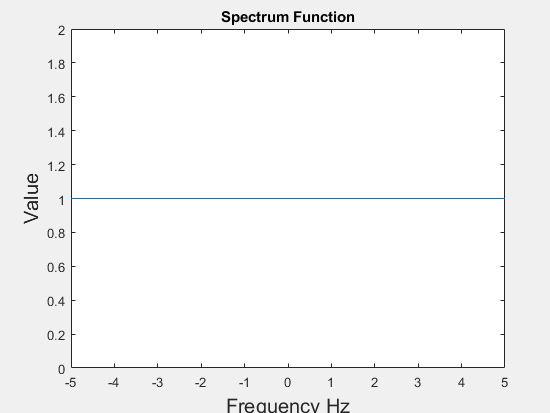
\includegraphics[scale=0.9]{images/spectrumfunct.png}
  \caption{Spectrum Function of a Dirac Function.}
  \label{fig:scheme1}
\end{figure}




    \item What is the spectrum of a square function with period T?
    The square function is defined by the Equation \ref{eq:square}.
    \begin{equation}
        G(x)=rect_{\tau} (t)
        \label{eq:square}
    \end{equation}
    In this way the spectrum is defined by \ref{eq:espectrumsquare}, Observing the equation in detail, it presents a sinusoidal or periodic behavior that is defined by the Fourier transform.
    \begin{equation}
        sinc(t)=\dfrac{ sin(\pi t)}{\pi * t}
        \label{eq:espectrumsquare}
    \end{equation}
    So that, the spectrum of this function is defined in the Figure \ref{fig:squarespec}, The spectrum of this function was found through the programming language, it is observable how according to the Fourier transform it respects the intrinsic behavior of the function.
    \begin{figure}[!h]
    \centering
  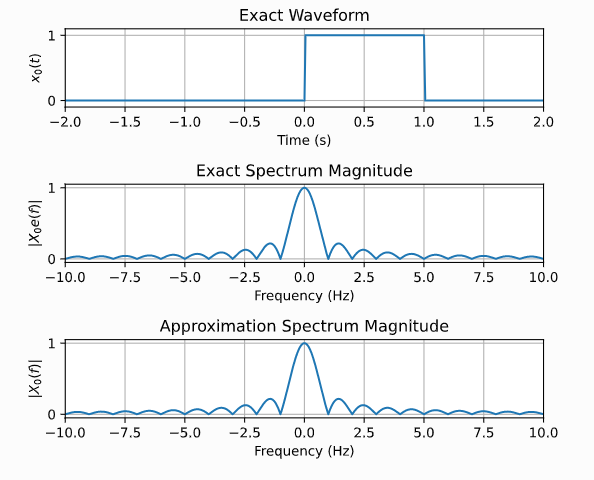
\includegraphics[scale=0.6]{images/squarespectrum.png}
  \caption{Spectrum Function of a Square Function.}
  \label{fig:squarespec}
    \end{figure}
    
    \item What is the spectrum of a pulse with rise time $\tau$ and duration T?
    The rise time of a pulse train is defined to be the length of time needed for the signal to transition from 0 to $\tau$, so to analyze the spectrum its better to observe the spectrum of a trapezoidal form which have a similar behavioral \cite{Bapfste}.
    \begin{figure}[!h]
    \centering
  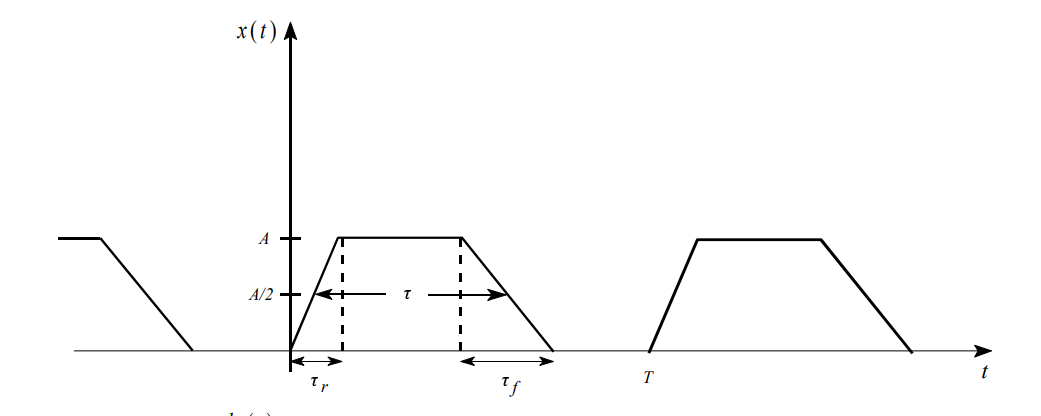
\includegraphics[scale=0.6]{images/Trapezoideal.png}
  \caption{Function of a Trapezoidal Function.}
  \label{fig:trap1}
    \end{figure}
    \begin{figure}[!h]
    \centering
  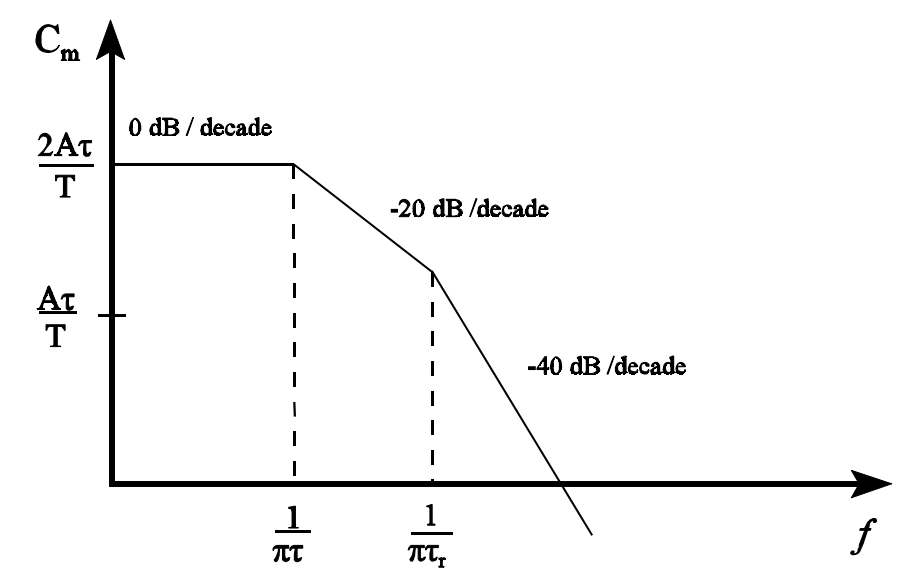
\includegraphics[scale=0.6]{images/Trapezoideal1.png}
  \caption{Spectrum Function of a Trapezoidal Function.}
  \label{fig:trap1a}
    \end{figure}
    So that, we observe in Figure \ref{fig:trap1}, that the spectrum of this function reaches a constant behavior in the area of increase, which is of interest in this question\footnote{\url{https://www.sciencedirect.com/topics/engineering/discrete-time-fourier-transform}}.
    \item What is the spectrum of a pulse with duration T gating a sine wave with frequency f, f $>>$ 1/T?
    Regarding the sinusoidal function that is intended to be found, it is possible to observe in Figure \ref{fig:sinusoideal}, where it is possible to observe how it reaches a response similar to the impulse, so it is assumed that Equation \ref{eq:phase} and \ref{eq:magintud} are used and the Fourier transform of such way to get these results.
    \begin{figure}[!h]
    \centering
  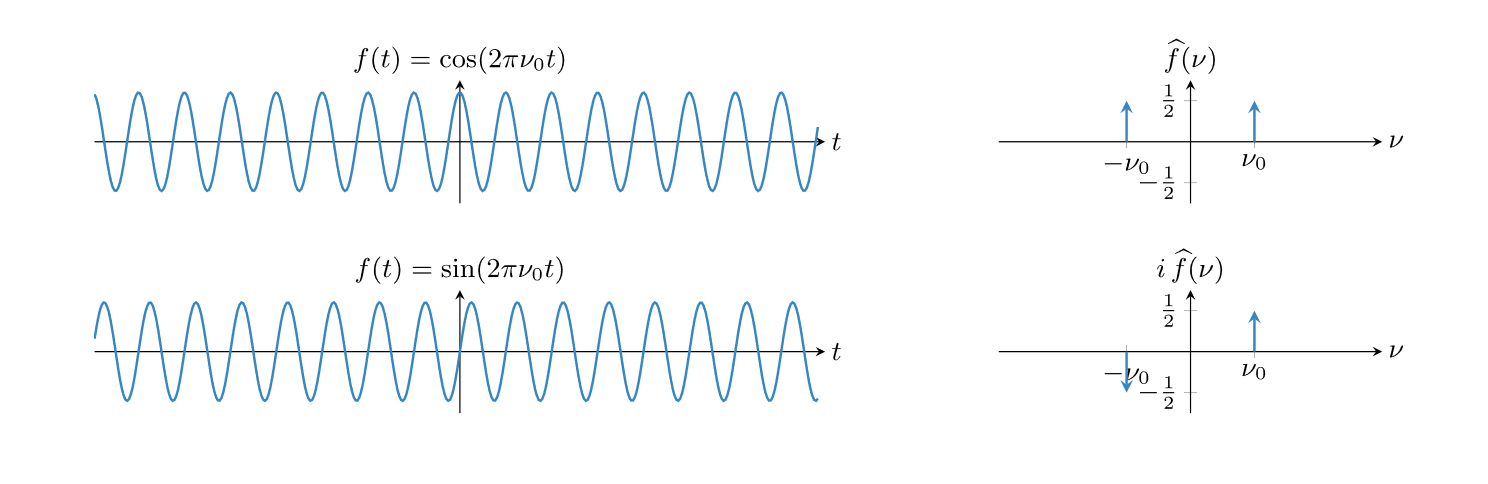
\includegraphics[scale=0.4]{images/sinusoideal.png}
  \caption{Spectrum Function of a Sinusoidal Function.}
  \label{fig:sinusoideal}
    \end{figure}
    
    
    
\end{itemize}


\enlargethispage{\baselineskip}
In this Project we developed and Application to an embedded digital network analyzer in order to obtain a embedded system with the possibility to measure external signals and develop the characterization, based in the previous works presented by Jean Michel Friedt in \cite{Friedt2021a} .\\

\chapter{Technical Section and Results}
In this chapter we will address and analyze the work developed in the weeks of development of the project, on the other hand the results found at the end of each section will also be shown and indicated. Finally, the implementation of each section is found in the attached Footnote\footnote{\url{https://github.com/GroverAruquipa/Embedded_digital_network_analyzer.git}}.
\section{First Week}
In order to start the first week the development of an application to an embedded digital network analyzer, we began by exploring the use of buidlroot (\cite{Abdullah2007}), the existing documentation on Linux bases was reviewed, in the same way using the build-essential package, these commands are well organized in the github repository attached, an eventually important recommendation is to be careful with the use of root and administrator tasks.\\

\begin{figure}[!h]
\centering
  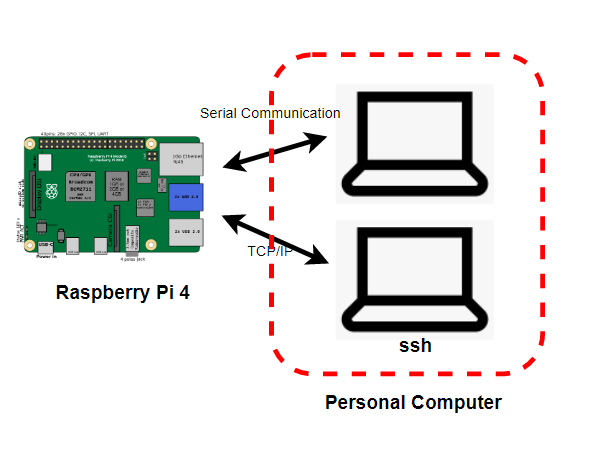
\includegraphics[scale=0.7]{images/scheme1a.png}
  \caption{Implementation scheme for the First week.}
  \label{fig:scheme1}
\end{figure}

Based on the previous paragraph in summary form, the following steps were carried out for the installation of GNURadio in an embedded system, in this case a Raspberry pi4.

\begin{figure}[!h]
\centering
  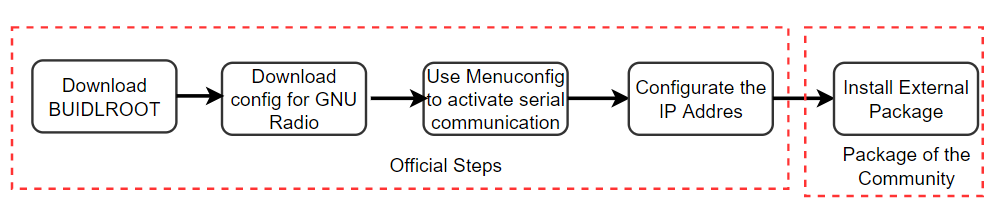
\includegraphics[width=\linewidth]{images/Steps1.png}
  \caption{Steps for the installation.}
  \label{fig:steps1}
\end{figure}
In the Figure \ref{fig:steps1} the summarized steps for the installation and use of GNURadio in embedded systems based on Linus are observed, in this way once downloaded and configured in Menuconfig, we proceed to make the configurations of the communication through Ethernet with the host or an external PC using Peer-to-Peer SSH. On the other hand, as specified, it is necessary to install extra libraries such as library \textit{rpitx} or \textit{pybombs} for the implementation of the blocks in the following weeks.\\
\newline
GNU radio greatly helps us develop radio frequency applications through a very simplified environment, without the need to directly access low-level coding in C or Python. The interface works under the QT framework, which makes it very flexible, easy to export, use external software developed by the community and in the same way the use of different visualization tools.
%%%%%%%%%%%%%%%%%%%%%%%%%%%%Additionally explanation equation
Thus, in an analog architecture there will be an antenna, a transducer, a reducer of frequency components, a signal processor to perform a transposition to the base band from 0Hz. Once we have a base band we can demodulate using a diode a to AM of a PLL for this case on FM signals, so the goal of using GNU Radio for this project is to replace all or most of these components with GNU-radio, which is stable and playable. Likewise, the analogy is shown in the following figure. Lastly, it is necessary to mention how GNU radio can easily handle the use of complex variables, which easily implies the use of terms such as phase and amplitude.
\begin{figure}[!h]
\centering
  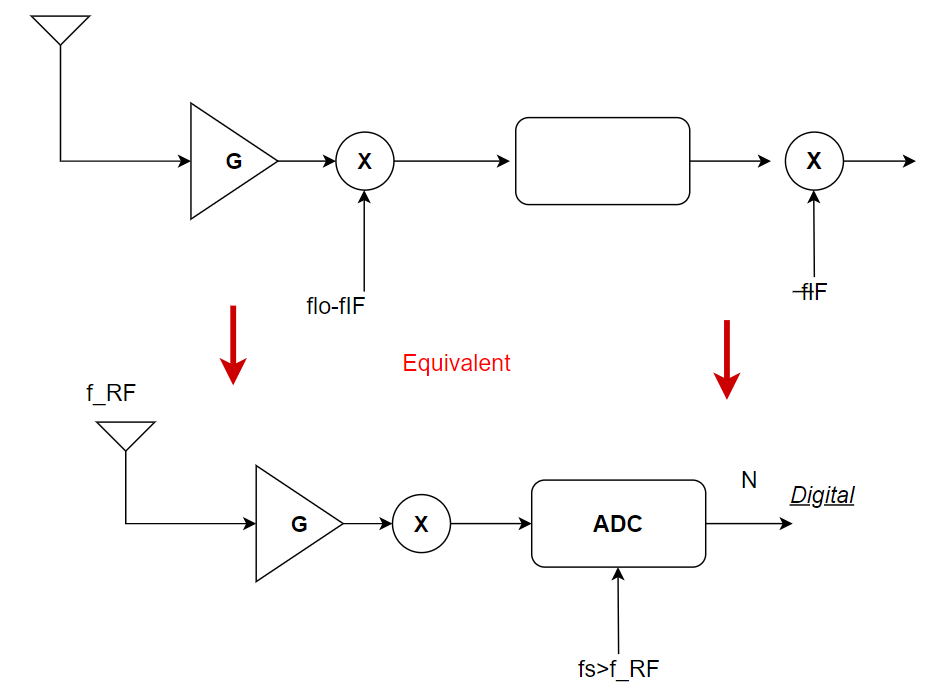
\includegraphics[width=\linewidth]{images/scheme1.png}
  \caption{Functional Scheme.}
  \label{fig:scheme1}
\end{figure}
In the  Figure \ref{fig:scheme1}, the signal will be send using the sampling frequency criterion where \textit{fs} must be greater than \textit{frf}, finally the quantization will be carried out with a given number of bits.
%%%%%%%%%%%%%%%%%%%%%%%explanation%%%%%%%%%%%%%%%%%%%%
So if we want to draw the spectrum, the band-with will be around \textit{Frf}, in such a way to correctly start the search and analysis of results, the concept of decimation was revised, which means that, through the given processor, we can only lose information, we cannot create it as such. So if we lose information we can reduce the bandwidth.\\ 
For example if we have a signal that goes from \textit{-fs/2} to \textit{fs/2} and we want to go in this range with a sample N of 1024, we can tell by a factor of D in the expression \textit{fs/2D} and \textit{fs/ND}, basically implies reducing the sampling time depending on the variable D, this example can be clearly shown in the following Figure \ref{fig:scheme1} . We must be very careful, because it can lead to aliasing problems that are the result of a periodic hypothesis in the spectrum, that is why to address this problem you must be sure to cancel it before the decimating, which gives us introduces what is the low pass filter.\\
Thus, based on the concepts explained above, the cutoff frequency of the low pass filter will be based on the range -fs/2D and fs/2D. Finally, to create an amplitude demodulation, two signal sources are necessary, which will help add the Carrier and the information to transmit.


%%%%%%%%%%%%%%%%%%%%%%%%%%%%%%%%%%%%%%%%%%%%%%%%%%%%%%%%%%%

\newpage
\section{Second Week}
In this week, concepts based primarily on the implementation of week 1 in a Raspberry pi 4 were explored, so for the beginning of this week the following scheme of use shown in Figure \ref{fig:scheme2} was used, the use of Ethernet communication through communication TCP/IP comes to have an added value in any project due mainly to the high advantages that it presents at the time of being implemented in a project from the standardization of sending packets either by TCP or UDP, the scalability in the use of different devices the ease of handling different types of messages we used the documentation available in the official document for this project \footnote{\url{http://jmfriedt.free.fr/hackable_buildroot.pdf}}\\
\begin{figure}[!h]
\centering
  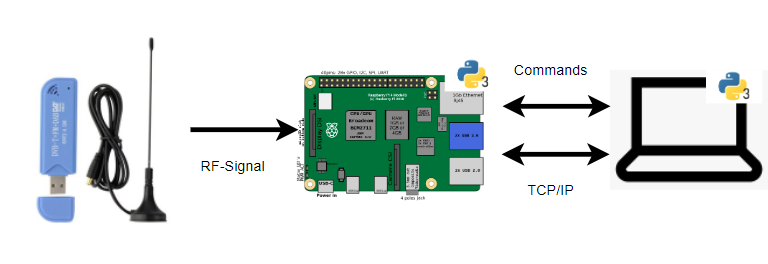
\includegraphics[width=\linewidth]{images/scheme_part2.png}
  \caption{Implementation scheme for the second week.}
  \label{fig:scheme2}
\end{figure}
\begin{figure}[!h]
\centering
  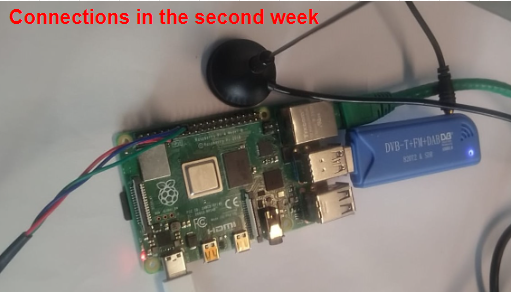
\includegraphics[width=\linewidth]{images/Conn_second.png}
  \caption{Connection for the experimentation in the Second week.}
  \label{fig:week2}
\end{figure}




On the other hand, the use of sockets is supported by the Python 3 language, which greatly facilitates data manipulation at the time of sending and receiving data, so this week the steps that were followed for the implementation are shown in Figure \ref{fig:scheme2a}.
\begin{figure}[!h]
\centering
  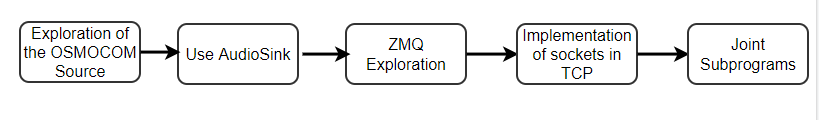
\includegraphics[width=\linewidth]{images/process2.png}
  \caption{Process of implementation for the second week.}
  \label{fig:scheme2a}
\end{figure}
In this specifically technical section, it is possible to observe how low-cost hardware is easily used for this project. At the beginning of the week, the first objective was the installation of GNU Radio, which entails an exploration of the use of native Linux and github commands, as well because the necessary support for the generation of the GNURadio image is found in the link $https://github.com/oscimp/oscimp_br2_external/tree/master/configs$ where it is possible to observe different configurations based on GNU Radio for the Raspberry pi, it should be noted that with the use of GNURadio 3.8 there is no need to install Pybombs.\\
Once the correct installation was done, it was necessary to carry out the verification by importing the library with the line of code :\textit{”import gnuradio”} in the Python IDLE of the Raspberry pi.\\ 
In order to explore \textit{GNURadio}, We can use GNU Radio in such a way to be able to observe its characterization in time and frequency that is shown in Figure \ref{fig:timefreq1}, so it is possible to see in this figure as through a cosine signal, we can easily see the spectrum of its signal.

\begin{figure}[!h]
\centering
  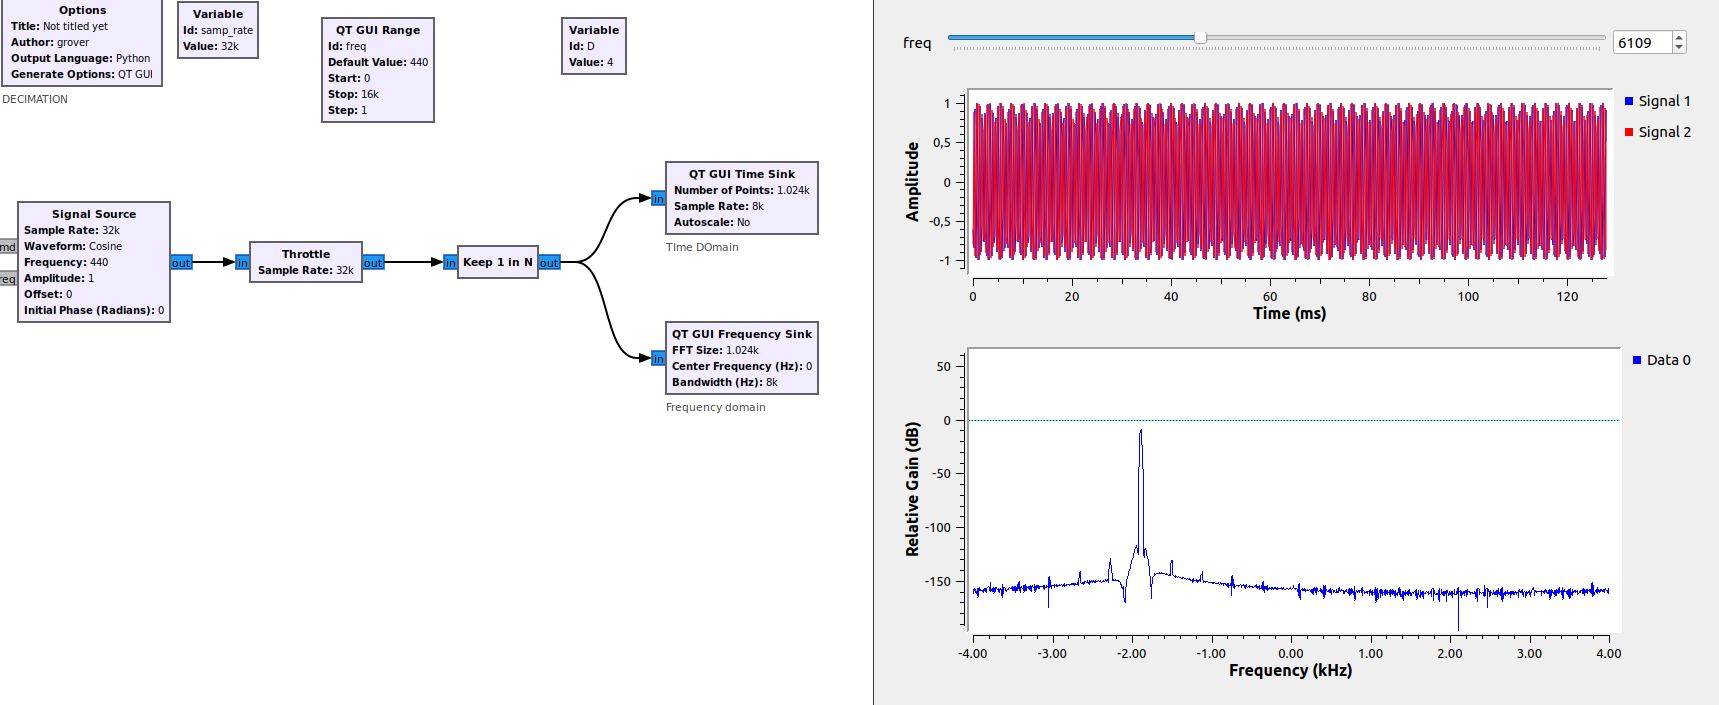
\includegraphics[width=\linewidth]{images/Frequency_time.png}
  \caption{First Exploration of GNURadio.}
  \label{fig:timefreq1}
\end{figure}
%%%%
Additionally, in order to be able to add components such as FIR or low-pass filters, the rapid design of filters is explored through the GNURadio design tool, it totally simplifies the total design, showing us components of frequency, magnitude and the position of poles and zeros, the which is shown in Figure \ref{fig:filterdes}.
\begin{figure}[!h]
\centering
  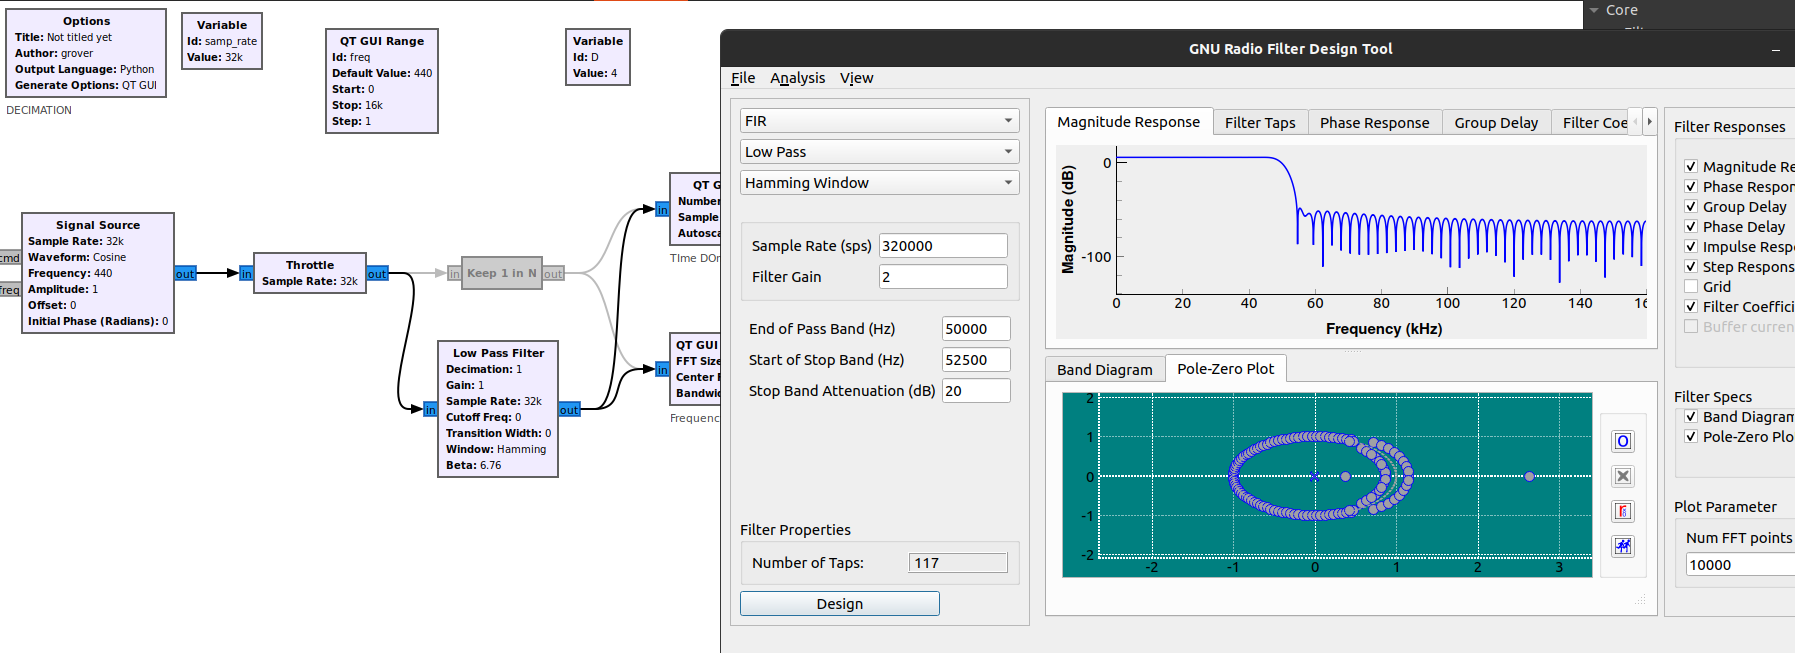
\includegraphics[width=\linewidth]{images/filter_design.png}
  \caption{Filter Designing.}
  \label{fig:filterdes}
\end{figure}
In the same way, once our filter has been characterized by means of the necessary cutoff frequency, it is possible to observe how we can characterize the FFT Avreage filter, in such a way as to obtain a correct value of change in the signal, shown in Figure \ref{fig:characteriz}, it can be Observe how the cutoff frequency is a function of the specified cutoff frequency. In the same way, it is observed how it is that a noisy signal was changed for the characterization of this filter, taking into account the decimation equal to 1.\\
\begin{figure}[!h]
\centering
  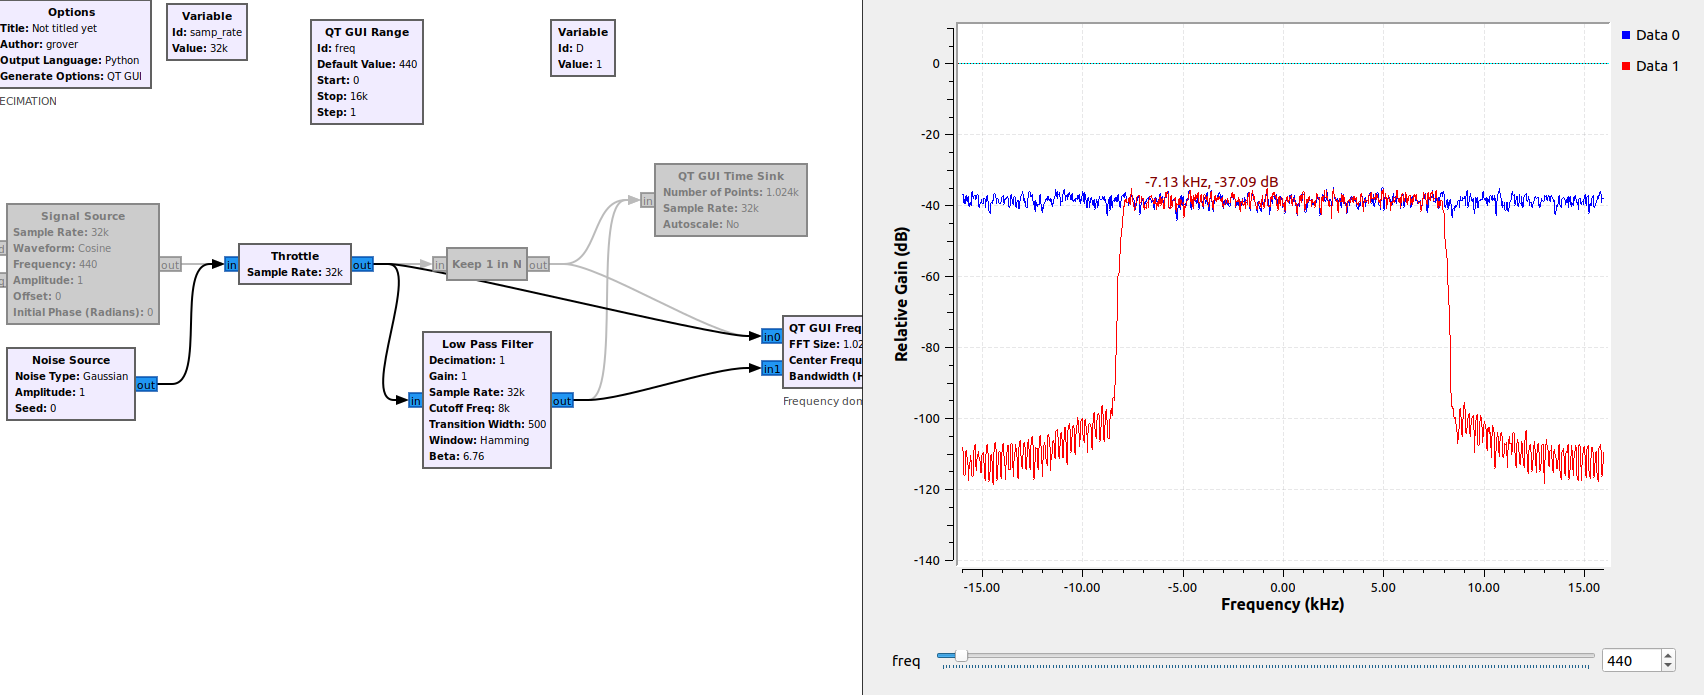
\includegraphics[width=\linewidth]{images/Frecuency_characterization.png}
  \caption{Filter Designing and Characterization.}
  \label{fig:characterization}
\end{figure}
%%%%

In this way, the use of a trivial example is made in the Host shown in figure \ref{fig:characterization}.
%%%%%%%%%%%%%%%%%%%%%%%%%%%%%A
In figure \ref{fig:firstsecond} it is possible to observe the use of a cosine-shaped signal with a frequency of 440, in this way this signal source is sent to the Audio Sink block, in the same way it is necessary to point out that to use it in the raspberry pi it must be omitted GUI support for Liberia functions. It is also necessary to note that the color of the orange connections imply a Float data type.\\
\begin{figure}[!h]
\centering
  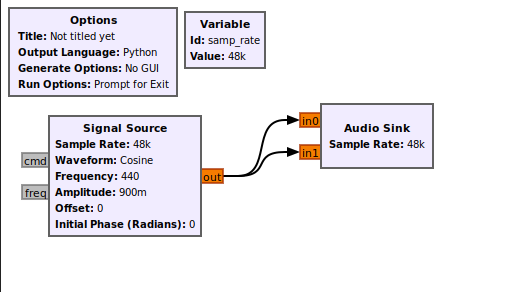
\includegraphics[width=\linewidth]{images/Program_1a.png}
  \caption{Audio output.}
  \label{fig:firstsecond}
\end{figure}
%%%%%B
On the other hand, Figure \ref{fig:hear} shows the use of the Osmocom block, which first goes through a low-pass filter, based on the explanation of the first week, it is interesting to note that in this program the variable block is used to be able to change the sample rate, this program.\\
This program has the objective of being able to change from listening to a radio frequency signal through the outputs of the raspberry pi, this program was used using the scp command for integration in the embedded card.\\
\begin{figure}[!h]
\centering
  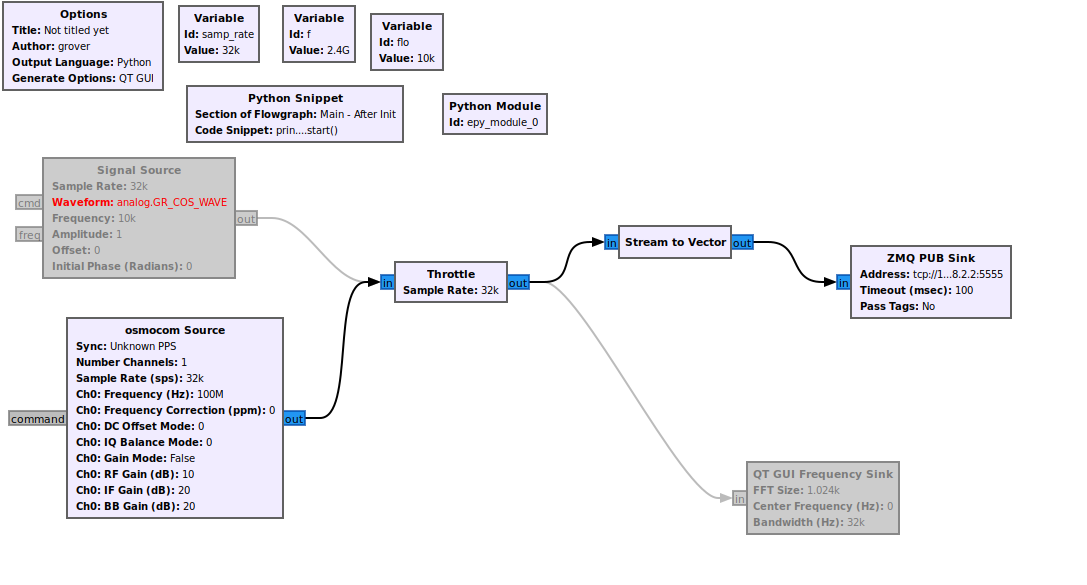
\includegraphics[width=\linewidth]{images/RPI_2WEEK.png}
  \caption{Raspberry pi Program for the Second Week.}
  \label{fig:RPISECONDWEEK}
\end{figure}


%%%%%%%%%%C
Continuing with this week's implementation For the streaming of the Demodulated FM signal on the Raspberry Pi4 to the PC with the sound card, the following block was used in Figure \ref{fig:LOCAL_HOST}, it is possible to observe the implementation of a local program in the PC, which is based on the following blocks diagram.\\
\begin{figure}[!h]
\centering
  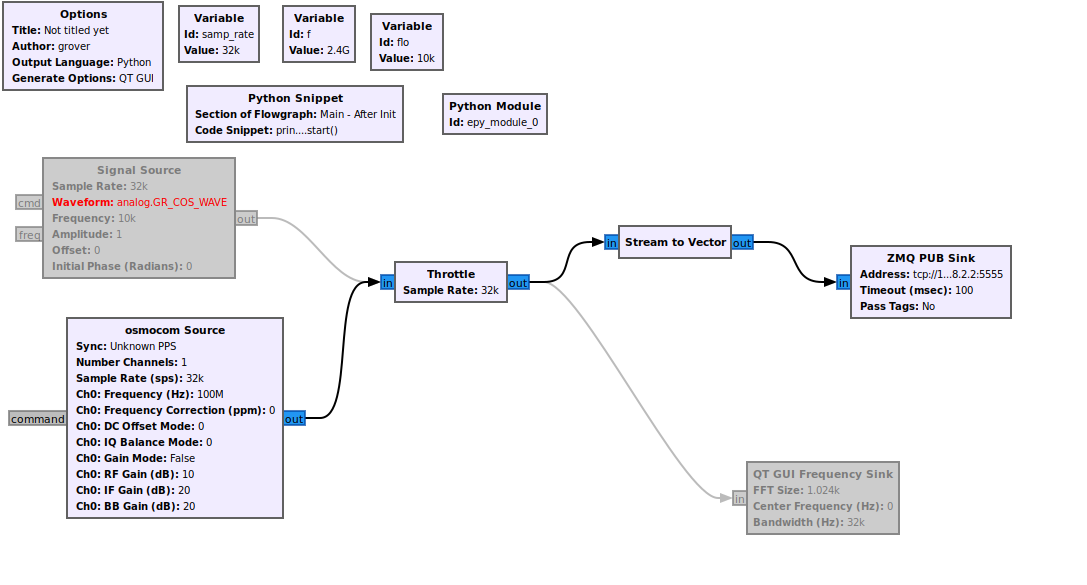
\includegraphics[width=\linewidth]{images/RPI_2WEEK.png}
  \caption{Local Host Diagram.}
  \label{fig:LOCAL_HOST}
\end{figure}

%%%D
Regarding Figure \ref{fig:LOCAL_HOST_TKIN}, it is necessary to point out that care should be taken when specifying the embedded IP and likewise the port of use.
From here for the final program, the use of threads was made for the communication between the server and the client, thus implying the sending of data streams to obtain the frequency path, based on the example code which was implemented in parallel. to the blocks shown above and combining them in such a way that the Raspberry pi can receive 4 different characters that are sent by the graphical interface developed in Python through Liberia Tkinter, which is shown in the repository attached to this report, additionally the interface to change the frequency in the raspberry pi using Ethernet is showed in the Figure\ref{fig:LOCAL_HOST_TKIN}.

\begin{figure}[!h]
\centering
  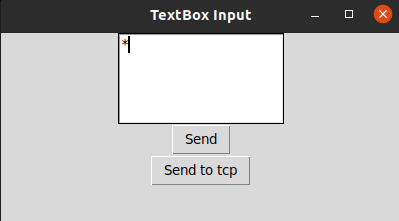
\includegraphics[width=\linewidth]{images/interfacea1.png}
  \caption{Local Interface, using Tkinter with Python.}
  \label{fig:LOCAL_HOST_TKINYER}
\end{figure}




%%%%%%%%%%%%%%%%%%%%%third week
%%%%%%%%%%%%%%%%%%%%%%%%%%%%%%%%%%%%

Then, at the end of week 2 and putting together the programs, the screen in Figure \ref{fig:intpro} is found following the previous steps, which represents the communication process between the client and the server.

\begin{figure}[!h]
\centering
  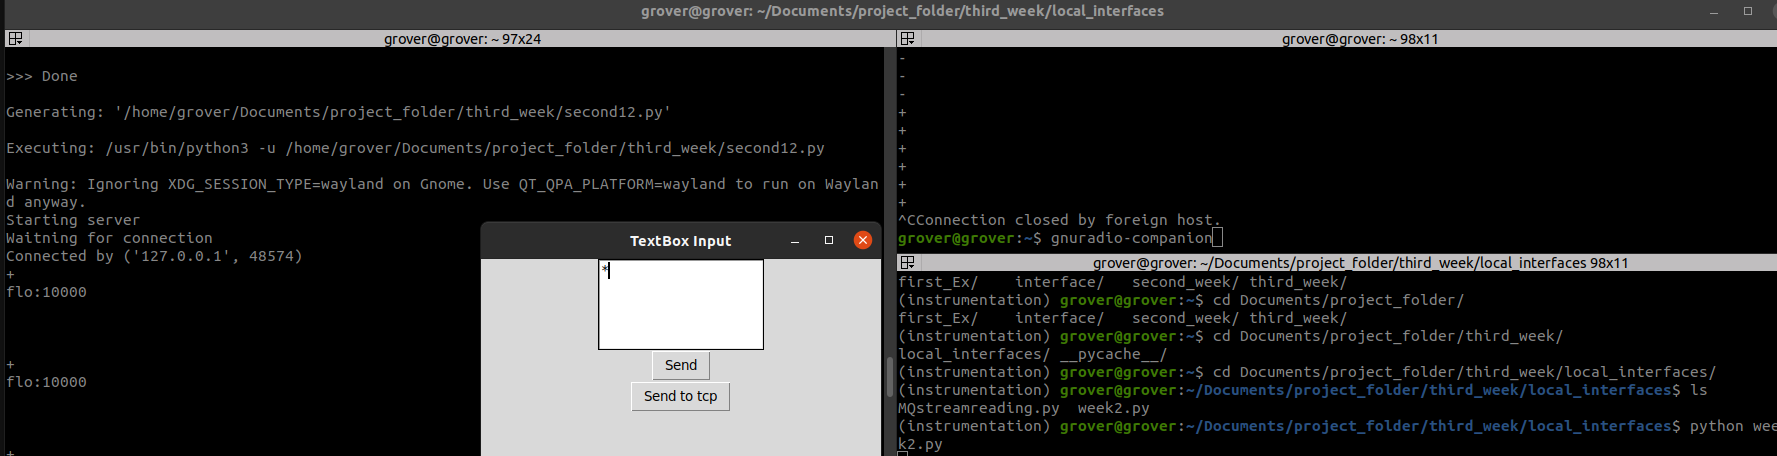
\includegraphics[width=\linewidth]{images/interface_fast.png}
  \caption{Interconnection of programs.}
  \label{fig:intpro}
\end{figure}


\section{Third Week}

In this week we research the radio frequency emissions using the internal PPL of the Raspberry pi4, feeding a GPIO as a radio frequency source. Thus ensuring that the radio frequency is controlled and understood using the DVT-T dongle based int he Figure \ref{fig:scheme3}. 
% Compile PiFM and its dependenciens for the RPi4
%% ADD FIGURE OF CONNEXTION OF THE WEEK OF WORK%%%%%%%%%%%%%%%%
\begin{figure}[!h]
\centering
  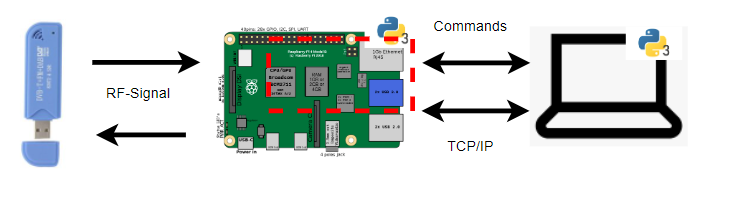
\includegraphics[width=\linewidth]{images/scheme3a.png}
  \caption{Implementation scheme for the third week.}
  \label{fig:scheme3}
\end{figure}
Additionally we can observe in the Figure \ref{fig:week3} its observable the scheme to connect the the physical system to find the necessary goals for the third week, in order to characterize the transfer function.  

\begin{figure}[!h]
\centering
  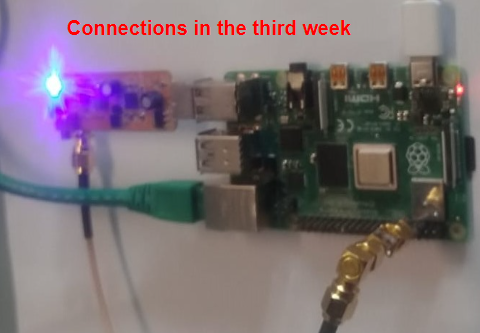
\includegraphics[width=\linewidth]{images/Conn_third.png}
  \caption{Connection for the experimentation in the Third week.}
  \label{fig:week3}
\end{figure}

%% %SOurces of radifrecuency%%%%%%%
RF waves in the physical environment are produced by different types of natural and artificial sources. For example in natural sources we can point out the sun, the earth and the ionosphere emit low level RF fields. In an application environment, artificial RF EMR sources are mainly used for telecommunication purposes in short or long distance systems. Radio and television broadcasts, mobile phones, wireless networks such as Wi-Fi, cordless phones, police and fire radios, point-to-point links, and satellite communications all produce RF EMR. Other sources of RF fields include microwave ovens, radars, industrial heaters and sealants, and various medical applications. \\
Thus, observing what was previously stated by the author, in this project we use a GPIO output from a Raspberry pi in order to obtain a radiation source. to be able to characterize it in the course of this chapter.\\
In order to obtain the correct experimental radio frequency power supply for the characterization of the signal, the internal PPL of the Raspberry pi is used, which will serve for the characterization of the signal. In this way, from the scheme shown above, the fractional PPL becomes governed by the following equations.\\

\begin{equation}
    VCO=LO X \frac{Q}{I}= \frac{LO}{I+F/4096}
    \label{equation:VCO}
\end{equation}
So that, to have an adequate use of the PPL, we take into account the equation \ref{equation:VCO} , where LO is the frequency provided by the 700 MHz clock for the Raspberry Pi4, additionally LO feeds the PPL \textit{(Phase Locked Loop)} with a pre scalar of I, also VCO times Q which is represented by $Q=\frac{1}{1+ F/4096/I}$, which is updated by $dQ=0.5^{12}$.On the other hand, the output frequency becomes less than 125Mhz with the use of an overtone in the 434Mhz FM band. For example for a 434 MHz we have a resolution of 0.45. \\%% !!!!!!!!!!!!ASK
This resolution becomes sufficient for this application or the characterization, due to the obtained value of dF, compared with a DDS, it is possible to observe a partial similarity to this structure, which helps the necessary understanding of this section.\\
%%%%%%%%%%%%%%%%Insert Image%%%%%%%%%%%%%%%%%%
Secondly, its necessary to identify the overtone, which will have the value based in the N scales as 1/N, so that emitted by 434/5=86.8MHz.\\
Thus, the FM reception and transmission from the raspberry pi to a HOST was first analyzed, which is implemented in GNU Radio, in this way the first generated Script is used in the embedded card or the Raspberry pi, which is responsible for acquisition, demodulation and streaming to the Host. On the other hand, there is also a script for the HOST which will be in charge of displaying the audio spectrum from the Raspberry pi. It is worth mentioning that in these two programs ZeroMQ is used, which is a high-performance message-oriented communications library, aimed at building distributed applications according to \cite{Simmonds2015}.\\
%%%%%%%%%%%Insert Image%%%%%%%%%%%%%
Thus, the following Figure \ref{fig:ZMQ1} shows the data received from here where it is observed how this signal is demodulated from the emission source, which is subsequently passed to a low-pass filter and sent through port 5555.\\
\begin{figure}[!h]
\centering
  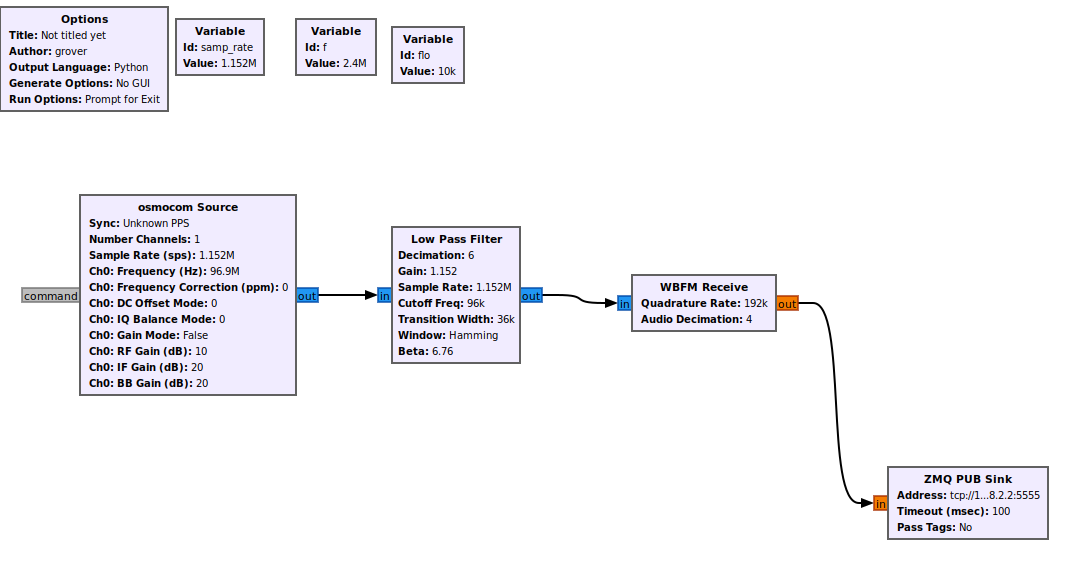
\includegraphics[width=\linewidth]{images/zmq pub.png}
  \caption{Using the ZMQ block.}
  \label{fig:ZMQ1}
\end{figure}
On the other hand, the SAW \textit{surface Accusative Wave} characterization should be carried out, so that  this device is connected in parallel to the external Antenna, this means its necessary disconnect the antenna when we start to measuring the SAW device to persuade the radiation problem and the collection of the noise.\\
In such way to make the use of the raspberry pi and their peripherals as such, the installation of the gr-rpitx library must be carried out, which is provided \footnote{\url{https://github.com/jmfriedt/gr-rpitx}}. 

This is an important to point out that when executing the steps necessary for the installation of this library according to the author unexpected installation events occur in the Ubuntu 20.04LTS distribution.\\ 
Which made it difficult and required a deep investigation of the use of Linux, due to the problem of the lack of library of \textit{liqdmasync.h}, Which was fixed by cross-compiling from a MINT-based Linux distribution.

\begin{figure}[!h]
\centering
  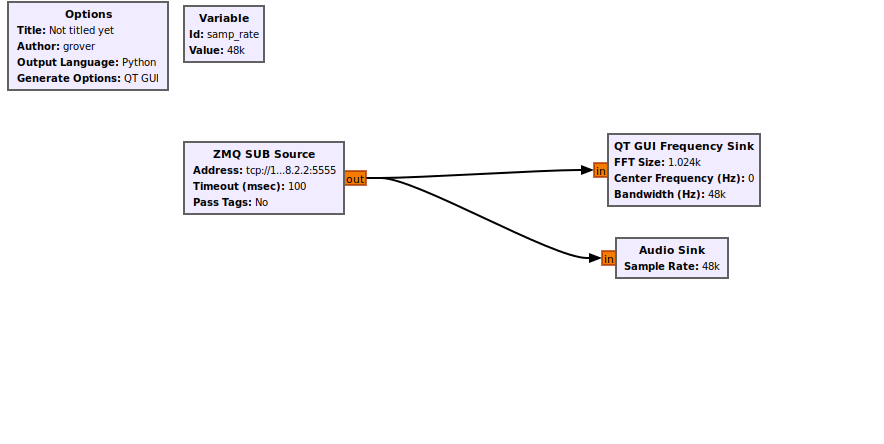
\includegraphics[width=\linewidth]{images/ZMQ_1A.png}
  \caption{Block for the reception.}
  \label{fig:ZMQ1}
\end{figure}

Figure \ref{fig:ZMQ1} shows the reception block that is used in the host, in this way the signal moved by the Raspberry pi is recovered, which will later help to characterize the signal, so it is necessary to point out that this is the configuration basis for characterizing the final transfer function.
\begin{figure}
     \centering
     \begin{subfigure}[b]{0.8\textwidth}
         \centering
         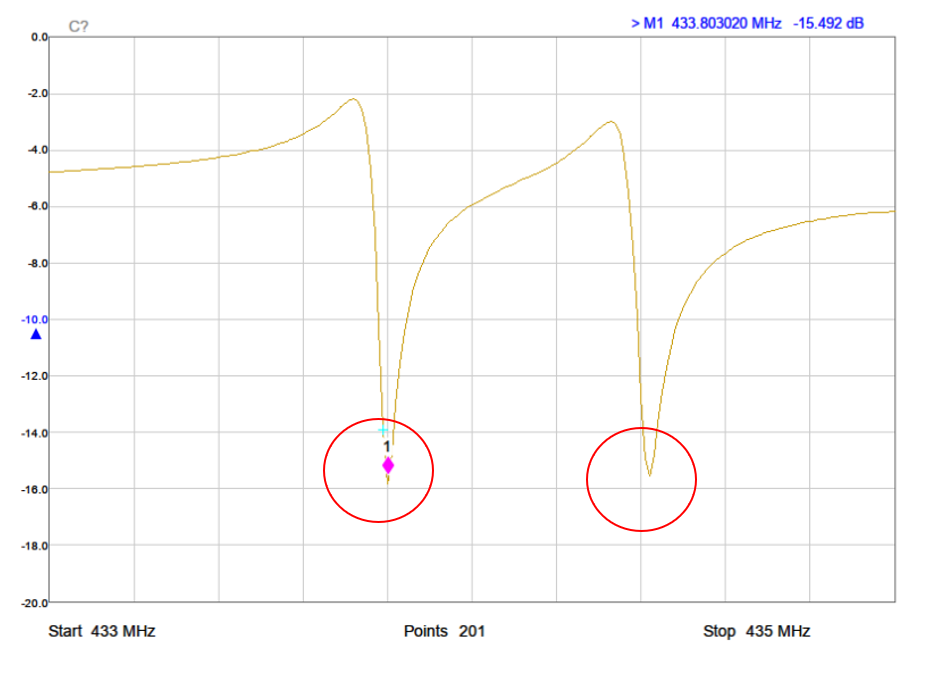
\includegraphics[width=\textwidth]{images/imr1.png}
         \caption{Limit 1 found by oscilloscope.}
         \label{fig:Osc1}
     \end{subfigure}
     \hfill
     \begin{subfigure}[b]{0.8\textwidth}
         \centering
         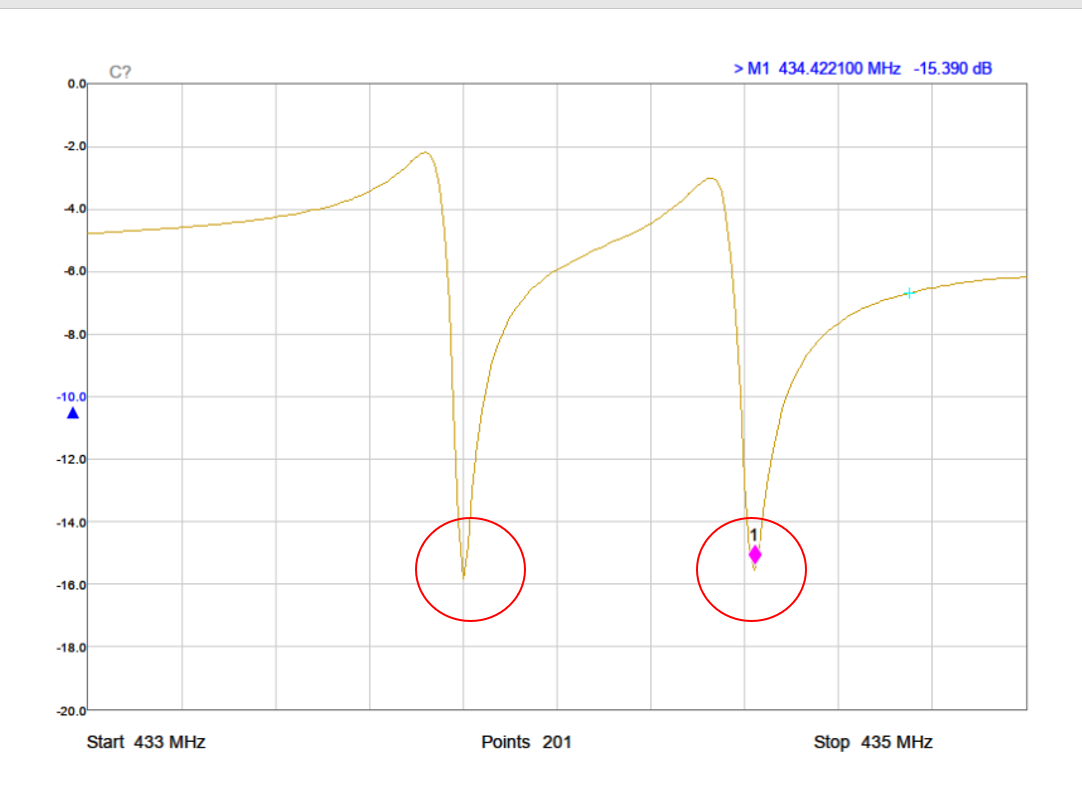
\includegraphics[width=\textwidth]{images/imr2.png}
         \caption{Limit 2 found by oscilloscope}
         \label{fig:Osc2}
     \end{subfigure}
     \hfill
        \caption{Finding the signal using the oscilloscope.}
        \label{fig:Osc}
\end{figure}
Prior to the characterization of the signal, it is possible to observe the output frequency of the system using an oscilloscope, which is shown in Figure \ref{fig:Osc} , through this signal we take the two important points that will serve as comparison, which are Frequency 1 and 2 shown in figures \ref{fig:Osc1} and \ref{fig:Osc2}.
%%%%
\begin{figure}
     \centering
     \begin{subfigure}[b]{0.8\textwidth}
         \centering
         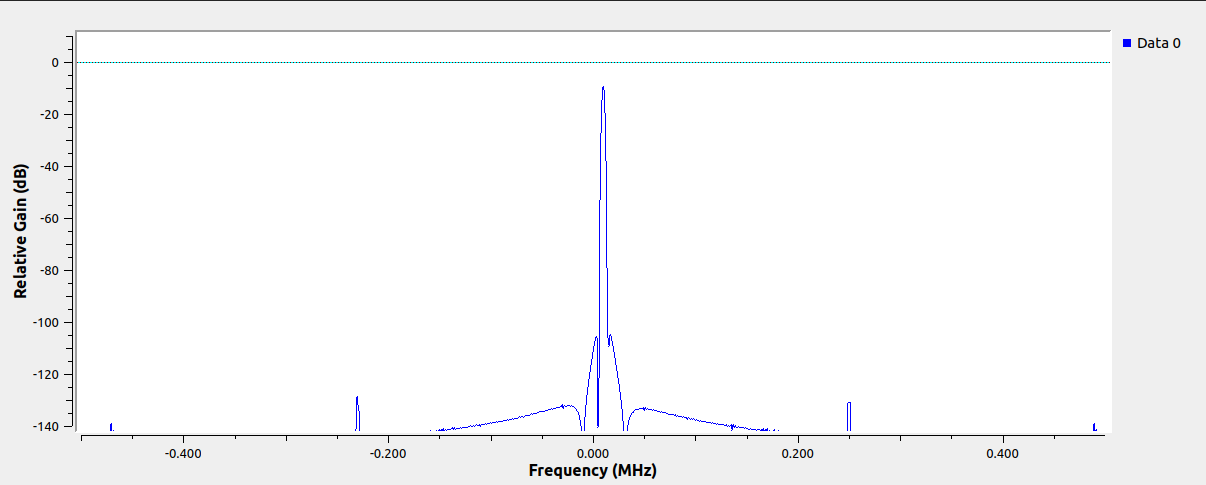
\includegraphics[width=\textwidth]{images/peak1a.png}
         \caption{First Peak found}
         \label{fig:Peak1}
     \end{subfigure}
     \hfill
     \begin{subfigure}[b]{0.8\textwidth}
         \centering
         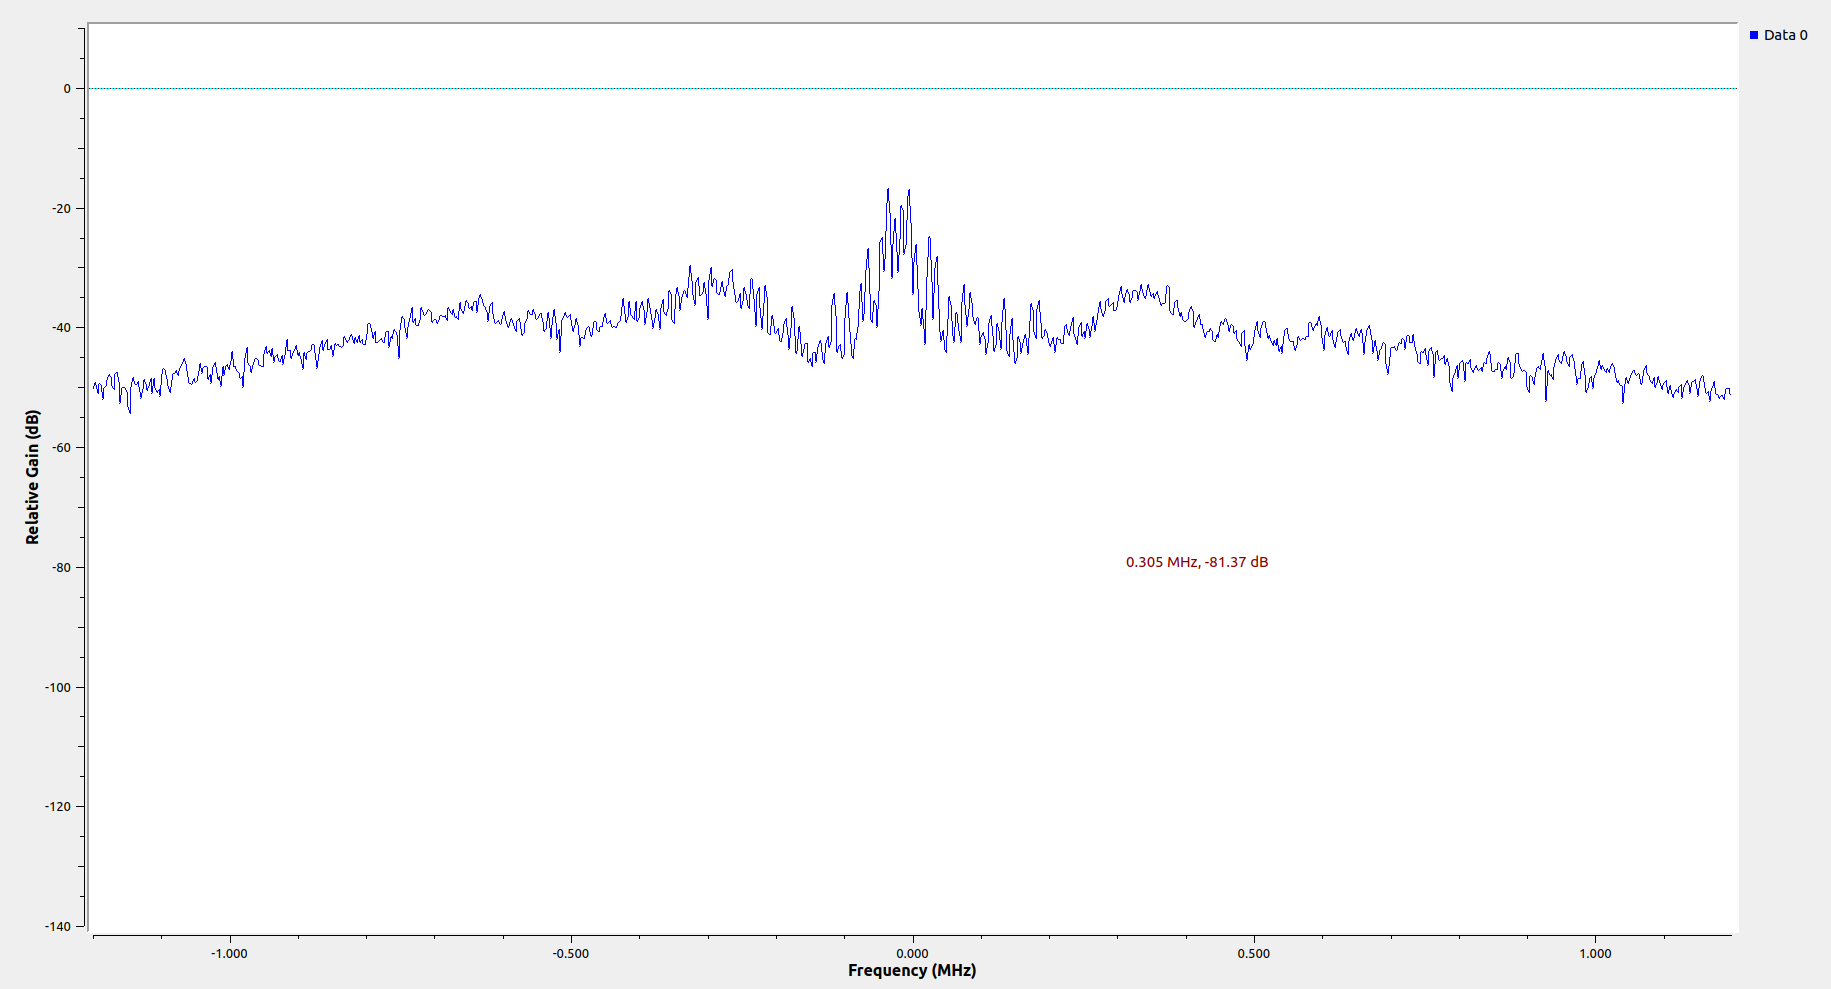
\includegraphics[width=\textwidth]{images/peak1.png}
         \caption{Second spike found}
         \label{fig:Peak2}
     \end{subfigure}
     \hfill
        \caption{Finding the Peaks.}
        \label{fig:Peaks}
\end{figure}




%% cOMMENT
Later we modified the script developed in week 2 that helps to obtain magnitude and phase, firstly a signal source was used which later had to be replaced by a source of collection in order to obtain the response in its module, the configuration of these blocks is observed on the Figure \ref{fig:ZMQ1}.
\begin{figure}[!h]
\centering
  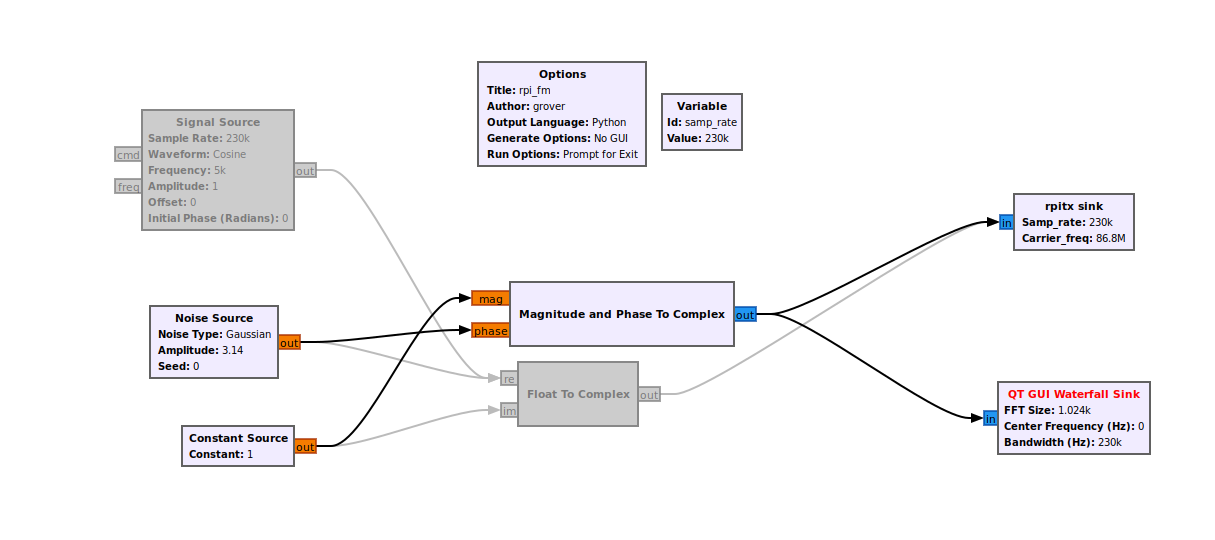
\includegraphics[width=\linewidth]{images/noise_3.png}
  \caption{Using the blocks for the characterization.}
  \label{fig:ZMQ1q}
\end{figure}
In this way, to finish, the desired data of the theoretical characterization of Frequency were found, which are shown in Figure \ref{fig:three graphs}, in this way it is observable that the frequency values sought are close to the theoretical ones.

\begin{figure}
     \centering
     \begin{subfigure}[b]{0.8\textwidth}
         \centering
         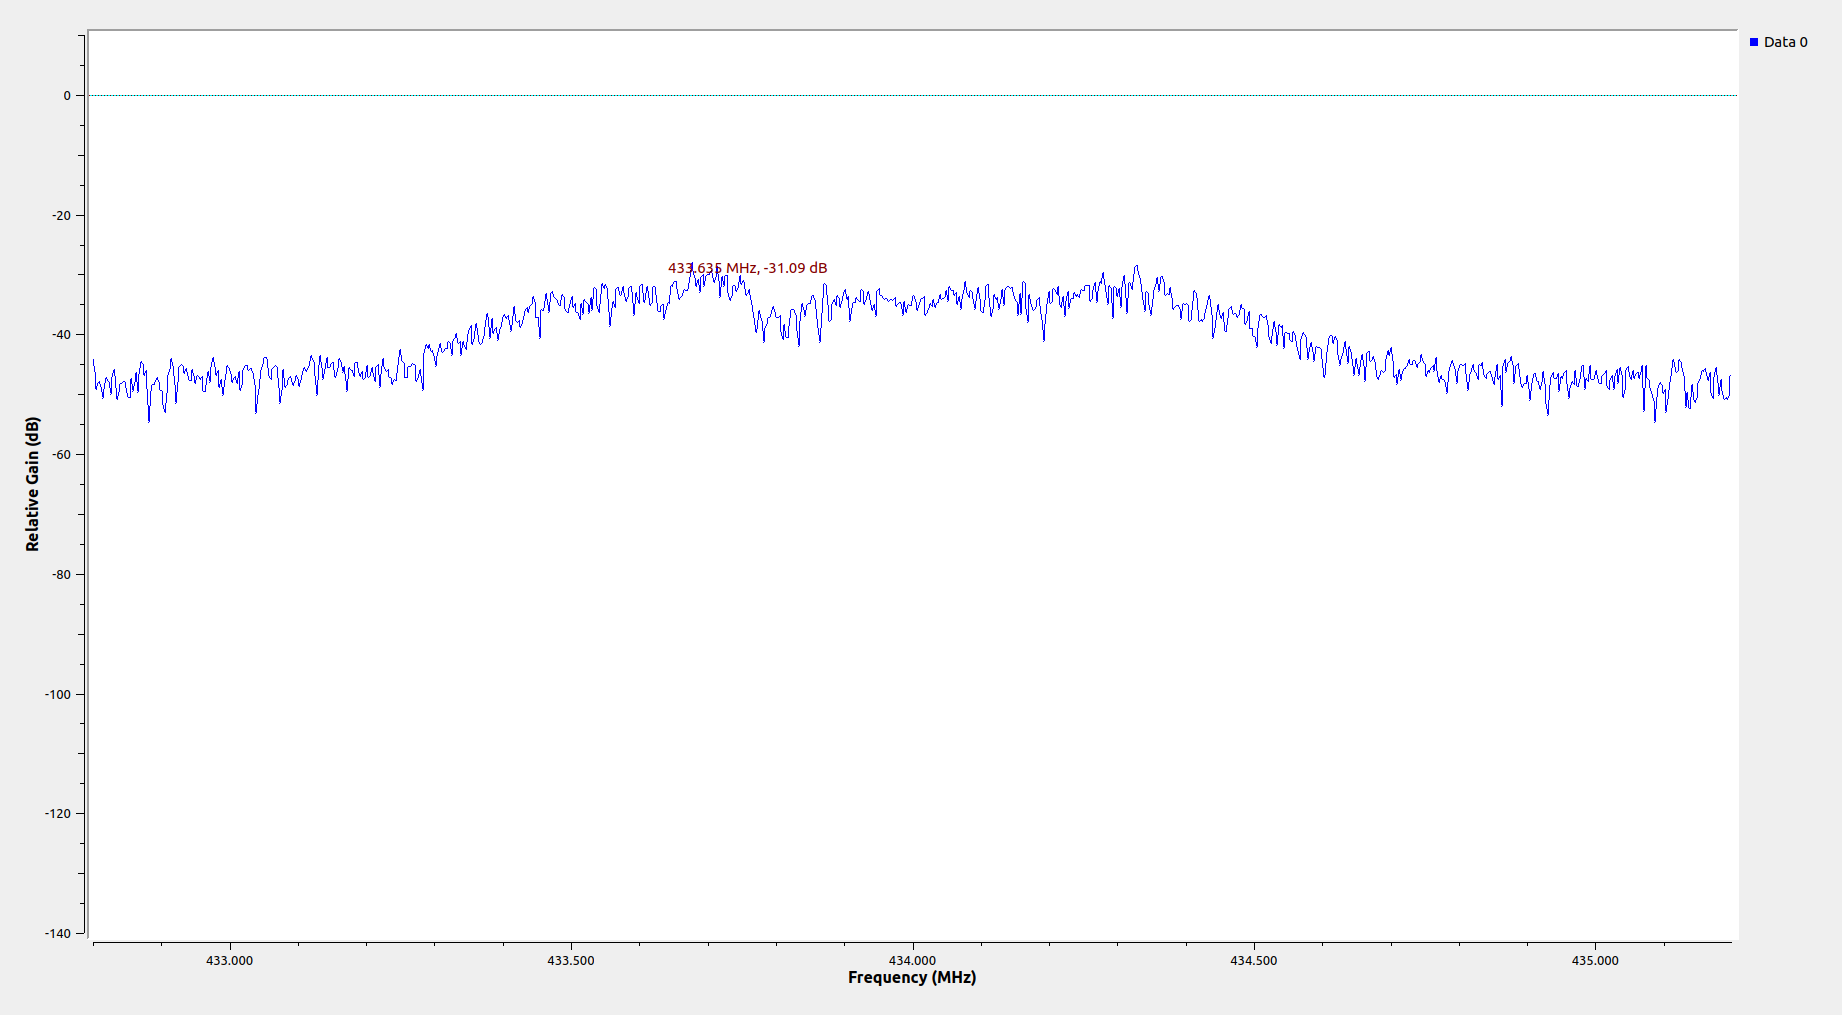
\includegraphics[width=\textwidth]{images/result1.png}
         \caption{Initial limit found}
         \label{fig:Result1}
     \end{subfigure}
     \hfill
     \begin{subfigure}[b]{0.8\textwidth}
         \centering
         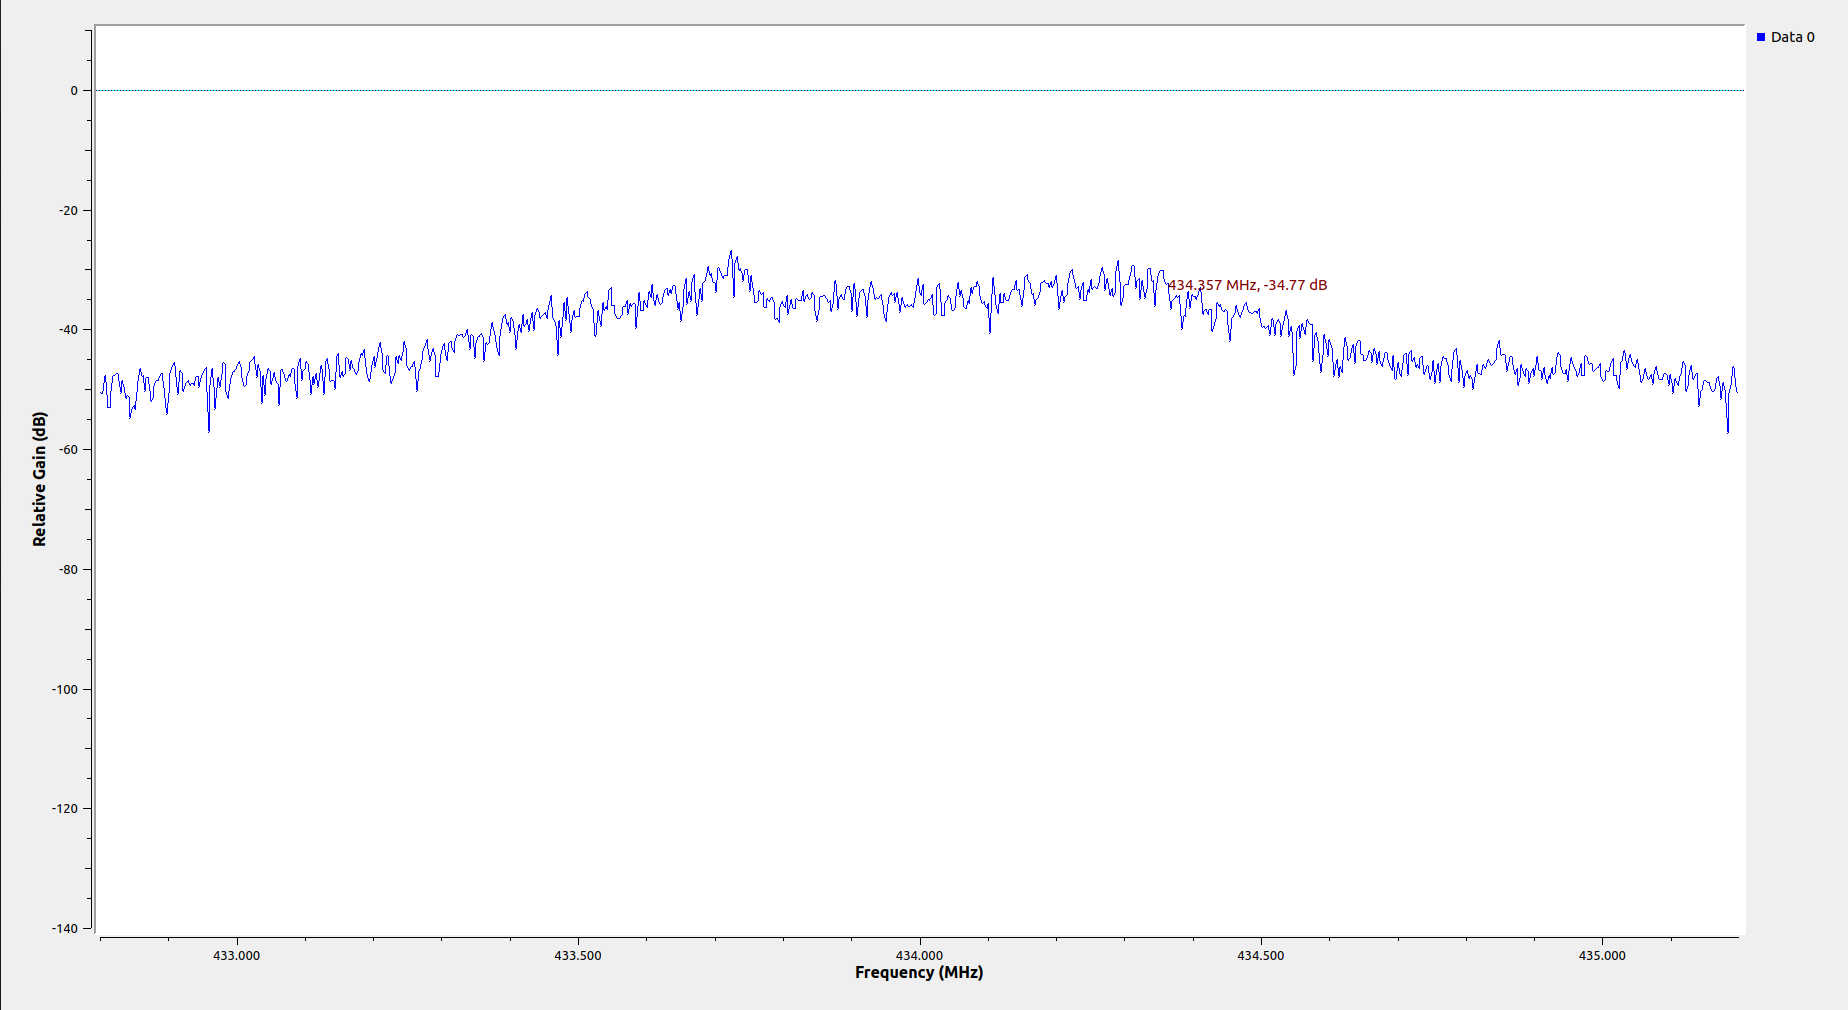
\includegraphics[width=\textwidth]{images/result2.png}
         \caption{Final limit found}
         \label{fig:Result2}
     \end{subfigure}
     \hfill
        \caption{Characterization of the signal.}
        \label{fig:three graphs}
\end{figure}

Although we can additionally add limitations when changing the frequency through the interface developed in the second week, the range of the frequencies According to the results found previously, it is 411.7 MHz and 434.4MHz, to find the correct frequency range we must consider that the signal range will be $[433.7MHz/5 ; 434.4MHz/5]$, then the ideal would be to add a condition in the base code used in order to respect these frequencies. The installation problems  which greatly limited the time available to develop it from the last part, showing partial results at the end of this report.

    
\chapter{Conclusion}
This practical work presented several sections that were contemplated previously, it is necessary to point out that although the objectives were not rigorously fulfilled in their entirety, the use and management of these tools oriented to research fields of a personal affinity such as the development of embedded systems for machine learning with the aim of having a greater optimization, in the same way it is necessary to mention that in the radio frequency part related applications such as remote control of \textit{cubesat's U1} or remote control by means of radio frequency were personally explored and GNU-Radio of mobile systems, thus observing the global impact of GNU-Radio, on the other hand the ease of GNU-Radio at the time of implementation is highlighted, it is easily comparable as the code generation simplifies the curve learning of different frameworks and necessary libraries, for example in [4] the author shows to the development of GNU-Radio blocks for the use of time series based on machine learning.\\
The expected results of the first week show a direct familiarization with \textit{buildroot} and embedded systems in \textit{SoC's}, it is possible to see how in this week the different configurations, the exploration and the use of Linux commands for this section were carried out, in the same way the obtaining quick sound by the \textit{Raspberry pi}. On the other hand, in week two the technical part of handling GNU-Radio was further developed, it is highlighted that in this section it is possible to implement a basic interface based on tkinter and \textit{TCP/IP}, through Ethernet Peer to peer. The tasty thing about this week was the management and change of frequency by sending commands, which can easily be extrapolated to different applications.\\
On the other hand, in week 3, the characterization of the transfer function was directly observed, although it is necessary to say that in this week the proposed objectives were partially met, this is due to third-party problems caused by the operating system. when compiling the \textit{rpitx} external Library, which was fixed by cross-compiling with a different Linux distribution.\\
The results shown at the end of this work partially reflect the objectives achieved, it is necessary to point out that the attached video in the \textit{github} repository clearly shows these results in a correctly explained way, so through the characterization of the transfer function the results are clearly observed. limits of the cutoff frequencies, which is comparable to the theoretical value sought and consequently validated, the manipulation and limits part was partially developed, not fully achieving this objective until the date of presentation of this report, for which it is not presented, in its entirety in your document.
\medskip
\chapter{Acknowledgment}
Acknowledgment and thanks principally to Professor Jean Michael Friedt for his great patience at the time of teaching and in the same way for the challenges he proposes not only to pass an exam but to really learn something and seek to apply or extrapolate it in areas of interest. In the same way towards Professor Franck Cholet for the guidelines of reporting and accompaniment in the formation of the last year. Finally, to my colleague Nelson Cisneros, a researcher on FEMTO-ST, for his valuable recommendations.
\cite{Wang2004}
\cite{Alfano2013}
\cite{Huang1991} 
\cite{Rao2015}
\cite{Yaqoob2005}
\cite{Kishi2016}
\cite{Ali2010}
\cite{Lee2014}
\cite{Izatt2008}
\cite{Hedrick2005}
\cite{Ourak2018}
\cite{Makita2017}
\cite{Cho2007}
\cite{Omar2006}
\cite{Liang2008}
\cite{Magerand2014} 
\cite{Bouma2004}
\cite{Pircher2007}
\cite{Pappuru2012}
\cite{Zawadzki2007}
\cite{Nocedal2006} 
\cite{Sakamoto2008}
\cite{Ricco2009}
\cite{D.Sampson}

\pagenumbering{gobble}

\printbibliography

\end{document}